\chapter{Najkraći putovi}

\index{najkraći put}

Pronalaženje najkraćeg puta između dva čvora
grafa
važan je zadatak koji ima mnogo
praktičnih primjena.
Na primjer, prirodan zadatak vezan uz cestovnu mrežu
jest izračunati najmanju moguću duljinu rute
između dvaju gradova, uz zadane duljine cesta.

U netežinskom grafu duljina puta jednaka je
broju njegovih bridova, pa možemo
jednostavno upotrijebiti pretraživanje u širinu za pronalaženje
najkraćeg puta.
Međutim, u ovom se poglavlju bavimo
težinskim grafovima
u kojima su za pronalaženje najkraćih putova
potrebni
složeniji algoritmi.

\section{Bellman–Fordov algoritam}

\index{Bellman–Fordov algoritam}

\key{Bellman–Fordov algoritam}\footnote{Algoritam je nazvan po
R. E. Bellmanu i L. R. Fordu koji su ga neovisno objavili
1958. odnosno 1956. godine \cite{bel58,for56a}.} pronalazi
najkraće putove od početnog čvora do svih
čvorova grafa.
Algoritam može obraditi sve vrste grafova,
uz uvjet da graf ne sadrži
ciklus negativne duljine.
Ako graf sadrži negativni ciklus,
algoritam to može otkriti.

Algoritam prati udaljenosti
od početnog čvora do svih čvorova grafa.
Na početku je udaljenost do početnog čvora 0,
a udaljenost do svih ostalih čvorova beskonačna.
Algoritam smanjuje udaljenosti pronalazeći
bridove koji skraćuju putove sve dok više nije
moguće smanjiti nijednu udaljenost.

\subsubsection{Primjer}

Razmotrimo kako Bellman–Fordov algoritam
radi na sljedećem grafu:
\begin{center}
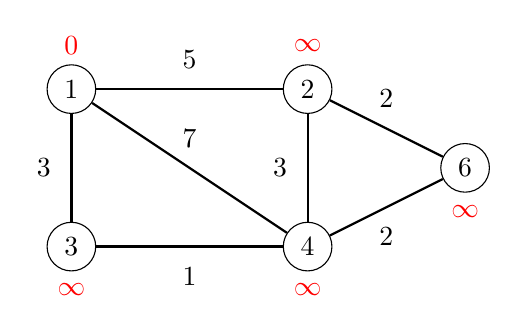
\begin{tikzpicture}
\node[draw, circle] (1) at (1,3) {1};
\node[draw, circle] (2) at (4,3) {2};
\node[draw, circle] (3) at (1,1) {3};
\node[draw, circle] (4) at (4,1) {4};
\node[draw, circle] (5) at (6,2) {6};
\node[color=red] at (1,3+0.55) {$0$};
\node[color=red] at (4,3+0.55) {$\infty$};
\node[color=red] at (1,1-0.55) {$\infty$};
\node[color=red] at (4,1-0.55) {$\infty$};
\node[color=red] at (6,2-0.55) {$\infty$};
\path[draw,thick,-] (1) -- node[font=\small,label=above:5] {} (2);
\path[draw,thick,-] (1) -- node[font=\small,label=left:3] {} (3);
\path[draw,thick,-] (3) -- node[font=\small,label=below:1] {} (4);
\path[draw,thick,-] (2) -- node[font=\small,label=left:3] {} (4);
\path[draw,thick,-] (2) -- node[font=\small,label=above:2] {} (5);
\path[draw,thick,-] (4) -- node[font=\small,label=below:2] {} (5);
\path[draw,thick,-] (1) -- node[font=\small,label=above:7] {} (4);
\end{tikzpicture}
\end{center}
Svakom je čvoru grafa pridružena udaljenost.
Na početku je udaljenost do početnog čvora 0,
a udaljenost do svih ostalih čvorova beskonačna.

Algoritam traži bridove koji smanjuju udaljenosti.
Najprije svi bridovi iz čvora 1 smanjuju udaljenosti:
\begin{center}
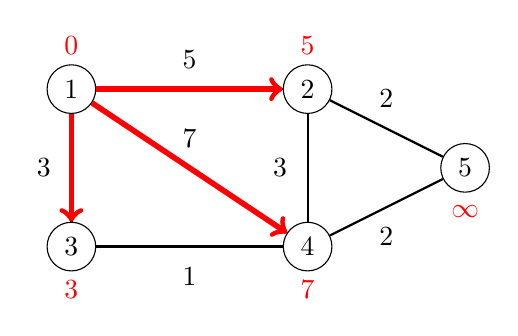
\begin{tikzpicture}
\node[draw, circle] (1) at (1,3) {1};
\node[draw, circle] (2) at (4,3) {2};
\node[draw, circle] (3) at (1,1) {3};
\node[draw, circle] (4) at (4,1) {4};
\node[draw, circle] (5) at (6,2) {5};
\node[color=red] at (1,3+0.55) {$0$};
\node[color=red] at (4,3+0.55) {$5$};
\node[color=red] at (1,1-0.55) {$3$};
\node[color=red] at (4,1-0.55) {$7$};
\node[color=red] at (6,2-0.55) {$\infty$};
\path[draw,thick,-] (1) -- node[font=\small,label=above:5] {} (2);
\path[draw,thick,-] (1) -- node[font=\small,label=left:3] {} (3);
\path[draw,thick,-] (3) -- node[font=\small,label=below:1] {} (4);
\path[draw,thick,-] (2) -- node[font=\small,label=left:3] {} (4);
\path[draw,thick,-] (2) -- node[font=\small,label=above:2] {} (5);
\path[draw,thick,-] (4) -- node[font=\small,label=below:2] {} (5);
\path[draw,thick,-] (1) -- node[font=\small,label=above:7] {} (4);

\path[draw=red,thick,->,line width=2pt] (1) -- (2);
\path[draw=red,thick,->,line width=2pt] (1) -- (3);
\path[draw=red,thick,->,line width=2pt] (1) -- (4);
\end{tikzpicture}
\end{center}
Nakon toga bridovi
$2 \rightarrow 5$ i $3 \rightarrow 4$
smanjuju udaljenosti:
\begin{center}
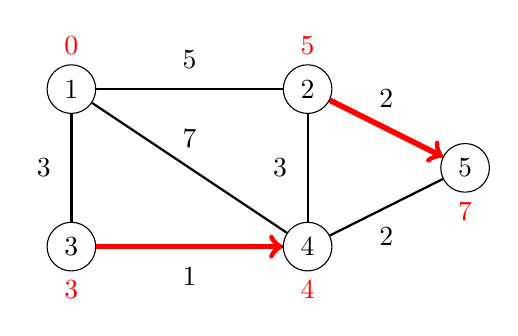
\begin{tikzpicture}
\node[draw, circle] (1) at (1,3) {1};
\node[draw, circle] (2) at (4,3) {2};
\node[draw, circle] (3) at (1,1) {3};
\node[draw, circle] (4) at (4,1) {4};
\node[draw, circle] (5) at (6,2) {5};
\node[color=red] at (1,3+0.55) {$0$};
\node[color=red] at (4,3+0.55) {$5$};
\node[color=red] at (1,1-0.55) {$3$};
\node[color=red] at (4,1-0.55) {$4$};
\node[color=red] at (6,2-0.55) {$7$};
\path[draw,thick,-] (1) -- node[font=\small,label=above:5] {} (2);
\path[draw,thick,-] (1) -- node[font=\small,label=left:3] {} (3);
\path[draw,thick,-] (3) -- node[font=\small,label=below:1] {} (4);
\path[draw,thick,-] (2) -- node[font=\small,label=left:3] {} (4);
\path[draw,thick,-] (2) -- node[font=\small,label=above:2] {} (5);
\path[draw,thick,-] (4) -- node[font=\small,label=below:2] {} (5);
\path[draw,thick,-] (1) -- node[font=\small,label=above:7] {} (4);

\path[draw=red,thick,->,line width=2pt] (2) -- (5);
\path[draw=red,thick,->,line width=2pt] (3) -- (4);
\end{tikzpicture}
\end{center}
Naposljetku, slijedi još jedna promjena:
\begin{center}
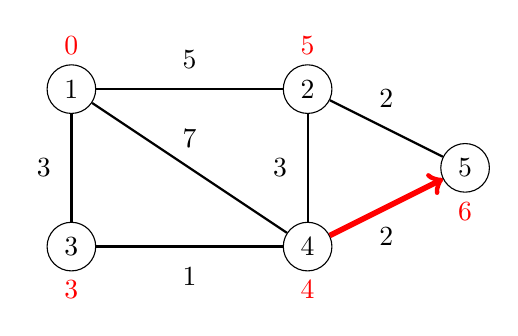
\begin{tikzpicture}
\node[draw, circle] (1) at (1,3) {1};
\node[draw, circle] (2) at (4,3) {2};
\node[draw, circle] (3) at (1,1) {3};
\node[draw, circle] (4) at (4,1) {4};
\node[draw, circle] (5) at (6,2) {5};
\node[color=red] at (1,3+0.55) {$0$};
\node[color=red] at (4,3+0.55) {$5$};
\node[color=red] at (1,1-0.55) {$3$};
\node[color=red] at (4,1-0.55) {$4$};
\node[color=red] at (6,2-0.55) {$6$};
\path[draw,thick,-] (1) -- node[font=\small,label=above:5] {} (2);
\path[draw,thick,-] (1) -- node[font=\small,label=left:3] {} (3);
\path[draw,thick,-] (3) -- node[font=\small,label=below:1] {} (4);
\path[draw,thick,-] (2) -- node[font=\small,label=left:3] {} (4);
\path[draw,thick,-] (2) -- node[font=\small,label=above:2] {} (5);
\path[draw,thick,-] (4) -- node[font=\small,label=below:2] {} (5);
\path[draw,thick,-] (1) -- node[font=\small,label=above:7] {} (4);

\path[draw=red,thick,->,line width=2pt] (4) -- (5);
\end{tikzpicture}
\end{center}

Nakon toga nijedan brid ne može smanjiti nijednu udaljenost.
To znači da su udaljenosti konačne
i da smo uspješno
izračunali najkraće udaljenosti
od početnog čvora do svih čvorova grafa.

Na primjer, najkraća udaljenost 3
od čvora 1 do čvora 5 odgovara
sljedećem putu:

\begin{center}
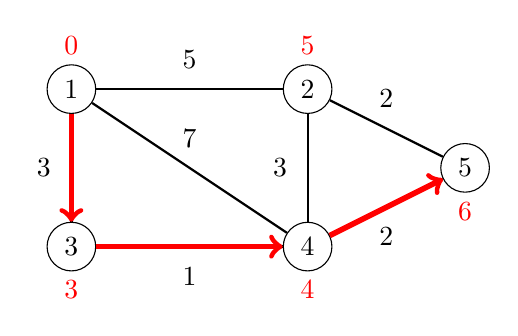
\begin{tikzpicture}
\node[draw, circle] (1) at (1,3) {1};
\node[draw, circle] (2) at (4,3) {2};
\node[draw, circle] (3) at (1,1) {3};
\node[draw, circle] (4) at (4,1) {4};
\node[draw, circle] (5) at (6,2) {5};
\node[color=red] at (1,3+0.55) {$0$};
\node[color=red] at (4,3+0.55) {$5$};
\node[color=red] at (1,1-0.55) {$3$};
\node[color=red] at (4,1-0.55) {$4$};
\node[color=red] at (6,2-0.55) {$6$};
\path[draw,thick,-] (1) -- node[font=\small,label=above:5] {} (2);
\path[draw,thick,-] (1) -- node[font=\small,label=left:3] {} (3);
\path[draw,thick,-] (3) -- node[font=\small,label=below:1] {} (4);
\path[draw,thick,-] (2) -- node[font=\small,label=left:3] {} (4);
\path[draw,thick,-] (2) -- node[font=\small,label=above:2] {} (5);
\path[draw,thick,-] (4) -- node[font=\small,label=below:2] {} (5);
\path[draw,thick,-] (1) -- node[font=\small,label=above:7] {} (4);

\path[draw=red,thick,->,line width=2pt] (1) -- (3);
\path[draw=red,thick,->,line width=2pt] (3) -- (4);
\path[draw=red,thick,->,line width=2pt] (4) -- (5);
\end{tikzpicture}
\end{center}

\subsubsection{Implementacija}

Sljedeća implementacija
Bellman–Fordova algoritma određuje najkraće udaljenosti
od čvora $x$ do svih čvorova grafa.
Kod pretpostavlja da je graf pohranjen
kao lista bridova \texttt{edges}
koja se sastoji od trojki oblika $(a,b,w)$,
što znači da postoji brid od čvora $a$ do čvora $b$
težine $w$.

Algoritam se sastoji od $n-1$ prolaza,
a u svakom prolazu algoritam prolazi kroz
sve bridove grafa i pokušava
smanjiti udaljenosti.
Algoritam gradi niz \texttt{distance}
koji će sadržavati udaljenosti od $x$
do svih čvorova grafa.
Konstanta \texttt{INF} označava beskonačnu udaljenost.

\begin{lstlisting}
for (int i = 1; i <= n; i++) distance[i] = INF;
distance[x] = 0;
for (int i = 1; i <= n-1; i++) {
    for (auto e : edges) {
        int a, b, w;
        tie(a, b, w) = e;
        distance[b] = min(distance[b], distance[a]+w);
    }
}
\end{lstlisting}

Vremenska složenost algoritma je $O(nm)$,
jer se algoritam sastoji od $n-1$ prolaza i
u svakom prolazu prolazi kroz svih $m$ bridova.
Ako u grafu nema negativnih ciklusa,
sve su udaljenosti konačne nakon $n-1$ prolaza,
jer svaki najkraći put može sadržavati najviše $n-1$ bridova.

U praksi se konačne udaljenosti obično
mogu pronaći brže nego u $n-1$ prolaza.
Stoga je jedan od načina da algoritam učinimo efikasnijim
zaustaviti ga ako se tijekom prolaza
nijedna udaljenost ne može smanjiti.

\subsubsection{Negativni ciklusi}

\index{negativni ciklus}

Bellman–Fordov algoritam može se upotrijebiti i za
provjeru sadrži li graf ciklus negativne duljine.
Na primjer, graf

\begin{center}
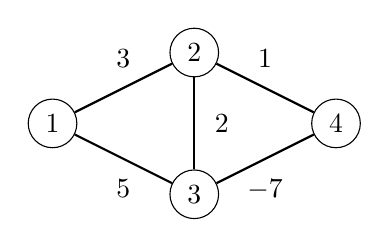
\begin{tikzpicture}[scale=0.9]
\node[draw, circle] (1) at (0,0) {$1$};
\node[draw, circle] (2) at (2,1) {$2$};
\node[draw, circle] (3) at (2,-1) {$3$};
\node[draw, circle] (4) at (4,0) {$4$};

\path[draw,thick,-] (1) -- node[font=\small,label=above:$3$] {} (2);
\path[draw,thick,-] (2) -- node[font=\small,label=above:$1$] {} (4);
\path[draw,thick,-] (1) -- node[font=\small,label=below:$5$] {} (3);
\path[draw,thick,-] (3) -- node[font=\small,label=below:$-7$] {} (4);
\path[draw,thick,-] (2) -- node[font=\small,label=right:$2$] {} (3);
\end{tikzpicture}
\end{center}
\noindent
sadrži negativni ciklus
$2 \rightarrow 3 \rightarrow 4 \rightarrow 2$
duljine $-4$.

Ako graf sadrži negativni ciklus,
svaki put koji sadrži taj ciklus možemo
skraćivati beskonačno mnogo puta ponavljajući ciklus
iznova i iznova.
Stoga pojam najkraćeg puta
u toj situaciji nema smisla.

Negativni ciklus možemo otkriti
Bellman–Fordovim algoritmom tako da
algoritam pokrenemo kroz $n$ prolaza.
Ako posljednji prolaz smanji neku udaljenost,
graf sadrži negativni ciklus.
Uočimo da se ovaj algoritam može upotrijebiti za
traženje
negativnog ciklusa u cijelom grafu,
neovisno o početnom čvoru.

\subsubsection{SPFA algoritam}

\index{SPFA algoritam}

\key{SPFA algoritam} (''Shortest Path Faster Algorithm'') \cite{fan94}
inačica je Bellman–Fordova algoritma
koja je često efikasnija od izvornog algoritma.
SPFA algoritam ne prolazi kroz sve bridove u svakom prolazu,
nego bridove koje će ispitati bira
na pametniji način.

Algoritam održava red čvorova koji bi se
mogli upotrijebiti za smanjivanje udaljenosti.
Najprije algoritam dodaje početni čvor $x$
u red.
Zatim algoritam uvijek obrađuje
prvi čvor u redu, a kada brid
$a \rightarrow b$ smanji udaljenost,
čvor $b$ dodaje se u red.
% 
% The following implementation uses a 
% \texttt{queue} \texttt{q}.
% In addition, an array \texttt{inqueue} indicates
% if a node is already in the queue,
% in which case the algorithm does not add
% the node to the queue again.
% 
% \begin{lstlisting}
% for (int i = 1; i <= n; i++) distance[i] = INF;
% distance[x] = 0;
% q.push(x);
% while (!q.empty()) {
%     int a = q.front(); q.pop();
%     inqueue[a] = false;
%     for (auto b : v[a]) {
%         if (distance[a]+b.second < distance[b.first]) {
%             distance[b.first] = distance[a]+b.second;
%             if (!inqueue[b]) {q.push(b); inqueue[b] = true;}
%         }
%     }
% }
% \end{lstlisting}

Efikasnost SPFA algoritma ovisi
o strukturi grafa:
algoritam je često efikasan,
ali je njegova vremenska složenost u najgorem slučaju i dalje
$O(nm)$ te je moguće konstruirati ulaze
zbog kojih algoritam postaje jednako spor kao
izvorni Bellman–Fordov algoritam.

\section{Dijkstrin algoritam}

\index{Dijkstrin algoritam}

\key{Dijkstrin algoritam}\footnote{E. W. Dijkstra objavio je algoritam 1959. godine \cite{dij59};
međutim, njegov izvorni rad ne spominje kako algoritam efikasno implementirati.}
pronalazi najkraće
putove od početnog čvora do svih čvorova grafa,
kao i Bellman–Fordov algoritam.
Prednost je Dijkstrina algoritma to što je
efikasniji i može se upotrijebiti za
obradu velikih grafova.
Međutim, algoritam zahtijeva da u grafu
nema bridova negativne težine.

Kao i Bellman–Fordov algoritam,
Dijkstrin algoritam održava udaljenosti
do čvorova i smanjuje ih tijekom pretraživanja.
Dijkstrin algoritam je efikasan jer
svaki brid grafa obrađuje
samo jednom, koristeći činjenicu
da nema negativnih bridova.

\subsubsection{Primjer}

Razmotrimo kako Dijkstrin algoritam
radi na sljedećem grafu kada je
početni čvor čvor 1:
\begin{center}
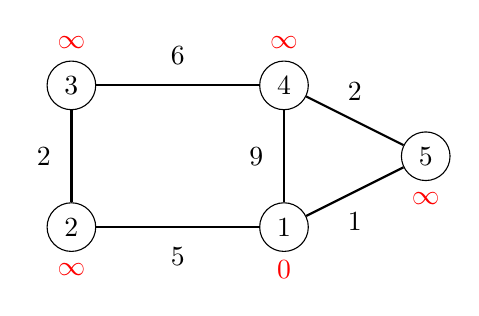
\begin{tikzpicture}[scale=0.9]
\node[draw, circle] (1) at (1,3) {3};
\node[draw, circle] (2) at (4,3) {4};
\node[draw, circle] (3) at (1,1) {2};
\node[draw, circle] (4) at (4,1) {1};
\node[draw, circle] (5) at (6,2) {5};

\node[color=red] at (1,3+0.6) {$\infty$};
\node[color=red] at (4,3+0.6) {$\infty$};
\node[color=red] at (1,1-0.6) {$\infty$};
\node[color=red] at (4,1-0.6) {$0$};
\node[color=red] at (6,2-0.6) {$\infty$};

\path[draw,thick,-] (1) -- node[font=\small,label=above:6] {} (2);
\path[draw,thick,-] (1) -- node[font=\small,label=left:2] {} (3);
\path[draw,thick,-] (3) -- node[font=\small,label=below:5] {} (4);
\path[draw,thick,-] (2) -- node[font=\small,label=left:9] {} (4);
\path[draw,thick,-] (2) -- node[font=\small,label=above:2] {} (5);
\path[draw,thick,-] (4) -- node[font=\small,label=below:1] {} (5);
\end{tikzpicture}
\end{center}
Kao i u Bellman–Fordovu algoritmu,
na početku je udaljenost do početnog čvora 0,
a udaljenost do svih ostalih čvorova beskonačna.

U svakom koraku Dijkstrin algoritam odabire čvor
koji još nije obrađen i čija je udaljenost
što manja.
Prvi takav čvor je čvor 1 s udaljenošću 0.

Kada je čvor odabran, algoritam
prolazi kroz sve bridove koji počinju u tom čvoru
i pomoću njih smanjuje udaljenosti:
\begin{center}
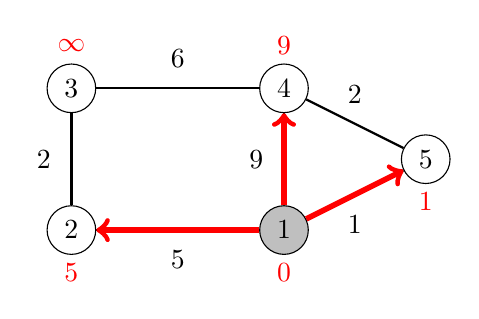
\begin{tikzpicture}[scale=0.9]
\node[draw, circle] (1) at (1,3) {3};
\node[draw, circle] (2) at (4,3) {4};
\node[draw, circle] (3) at (1,1) {2};
\node[draw, circle, fill=lightgray] (4) at (4,1) {1};
\node[draw, circle] (5) at (6,2) {5};

\node[color=red] at (1,3+0.6) {$\infty$};
\node[color=red] at (4,3+0.6) {$9$};
\node[color=red] at (1,1-0.6) {$5$};
\node[color=red] at (4,1-0.6) {$0$};
\node[color=red] at (6,2-0.6) {$1$};

\path[draw,thick,-] (1) -- node[font=\small,label=above:6] {} (2);
\path[draw,thick,-] (1) -- node[font=\small,label=left:2] {} (3);
\path[draw,thick,-] (3) -- node[font=\small,label=below:5] {} (4);
\path[draw,thick,-] (2) -- node[font=\small,label=left:9] {} (4);
\path[draw,thick,-] (2) -- node[font=\small,label=above:2] {} (5);
\path[draw,thick,-] (4) -- node[font=\small,label=below:1] {} (5);

\path[draw=red,thick,->,line width=2pt] (4) -- (2);
\path[draw=red,thick,->,line width=2pt] (4) -- (3);
\path[draw=red,thick,->,line width=2pt] (4) -- (5);
\end{tikzpicture}
\end{center}
U ovom su slučaju
bridovi iz čvora 1 smanjili udaljenosti
čvorova 2, 4 i 5, čije su udaljenosti sada 5, 9 i 1.

Sljedeći čvor koji se obrađuje je čvor 5 s udaljenošću 1.
Time se udaljenost do čvora 4 smanjuje s 9 na 3:
\begin{center}
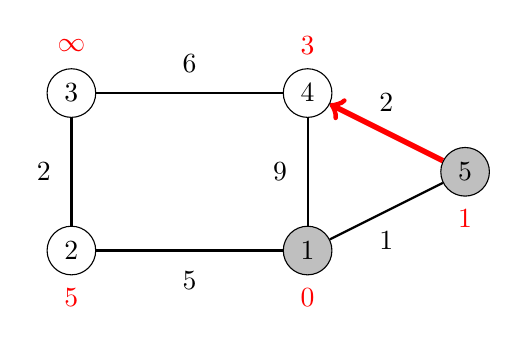
\begin{tikzpicture}
\node[draw, circle] (1) at (1,3) {3};
\node[draw, circle] (2) at (4,3) {4};
\node[draw, circle] (3) at (1,1) {2};
\node[draw, circle, fill=lightgray] (4) at (4,1) {1};
\node[draw, circle, fill=lightgray] (5) at (6,2) {5};

\node[color=red] at (1,3+0.6) {$\infty$};
\node[color=red] at (4,3+0.6) {$3$};
\node[color=red] at (1,1-0.6) {$5$};
\node[color=red] at (4,1-0.6) {$0$};
\node[color=red] at (6,2-0.6) {$1$};

\path[draw,thick,-] (1) -- node[font=\small,label=above:6] {} (2);
\path[draw,thick,-] (1) -- node[font=\small,label=left:2] {} (3);
\path[draw,thick,-] (3) -- node[font=\small,label=below:5] {} (4);
\path[draw,thick,-] (2) -- node[font=\small,label=left:9] {} (4);
\path[draw,thick,-] (2) -- node[font=\small,label=above:2] {} (5);
\path[draw,thick,-] (4) -- node[font=\small,label=below:1] {} (5);

\path[draw=red,thick,->,line width=2pt] (5) -- (2);
\end{tikzpicture}
\end{center}
Nakon toga na redu je čvor 4, koji smanjuje
udaljenost do čvora 3 na 9:
\begin{center}
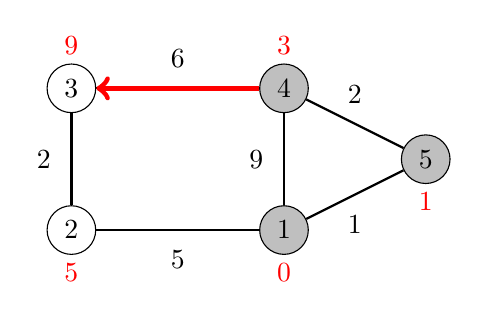
\begin{tikzpicture}[scale=0.9]
\node[draw, circle] (1) at (1,3) {3};
\node[draw, circle, fill=lightgray] (2) at (4,3) {4};
\node[draw, circle] (3) at (1,1) {2};
\node[draw, circle, fill=lightgray] (4) at (4,1) {1};
\node[draw, circle, fill=lightgray] (5) at (6,2) {5};

\node[color=red] at (1,3+0.6) {$9$};
\node[color=red] at (4,3+0.6) {$3$};
\node[color=red] at (1,1-0.6) {$5$};
\node[color=red] at (4,1-0.6) {$0$};
\node[color=red] at (6,2-0.6) {$1$};

\path[draw,thick,-] (1) -- node[font=\small,label=above:6] {} (2);
\path[draw,thick,-] (1) -- node[font=\small,label=left:2] {} (3);
\path[draw,thick,-] (3) -- node[font=\small,label=below:5] {} (4);
\path[draw,thick,-] (2) -- node[font=\small,label=left:9] {} (4);
\path[draw,thick,-] (2) -- node[font=\small,label=above:2] {} (5);
\path[draw,thick,-] (4) -- node[font=\small,label=below:1] {} (5);

\path[draw=red,thick,->,line width=2pt] (2) -- (1);
\end{tikzpicture}
\end{center}

Izvanredno je svojstvo Dijkstrina algoritma to da je
udaljenost čvora konačna čim je taj čvor odabran.
Na primjer, u ovom su trenutku algoritma
udaljenosti 0, 1 i 3 konačne udaljenosti
do čvorova 1, 5 i 4.

Nakon toga algoritam obrađuje preostala
dva čvora, a konačne su udaljenosti sljedeće:

\begin{center}
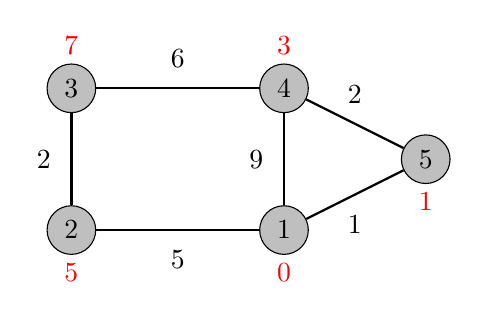
\begin{tikzpicture}[scale=0.9]
\node[draw, circle, fill=lightgray] (1) at (1,3) {3};
\node[draw, circle, fill=lightgray] (2) at (4,3) {4};
\node[draw, circle, fill=lightgray] (3) at (1,1) {2};
\node[draw, circle, fill=lightgray] (4) at (4,1) {1};
\node[draw, circle, fill=lightgray] (5) at (6,2) {5};

\node[color=red] at (1,3+0.6) {$7$};
\node[color=red] at (4,3+0.6) {$3$};
\node[color=red] at (1,1-0.6) {$5$};
\node[color=red] at (4,1-0.6) {$0$};
\node[color=red] at (6,2-0.6) {$1$};

\path[draw,thick,-] (1) -- node[font=\small,label=above:6] {} (2);
\path[draw,thick,-] (1) -- node[font=\small,label=left:2] {} (3);
\path[draw,thick,-] (3) -- node[font=\small,label=below:5] {} (4);
\path[draw,thick,-] (2) -- node[font=\small,label=left:9] {} (4);
\path[draw,thick,-] (2) -- node[font=\small,label=above:2] {} (5);
\path[draw,thick,-] (4) -- node[font=\small,label=below:1] {} (5);
\end{tikzpicture}
\end{center}

\subsubsection{Negativni bridovi}

Efikasnost Dijkstrina algoritma
temelji se na činjenici da graf ne
sadrži negativne bridove.
Ako postoji negativni brid,
algoritam može dati netočne rezultate.
Kao primjer, razmotrimo sljedeći graf:

\begin{center}
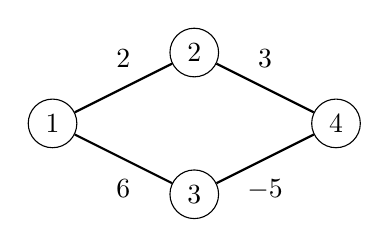
\begin{tikzpicture}[scale=0.9]
\node[draw, circle] (1) at (0,0) {$1$};
\node[draw, circle] (2) at (2,1) {$2$};
\node[draw, circle] (3) at (2,-1) {$3$};
\node[draw, circle] (4) at (4,0) {$4$};

\path[draw,thick,-] (1) -- node[font=\small,label=above:2] {} (2);
\path[draw,thick,-] (2) -- node[font=\small,label=above:3] {} (4);
\path[draw,thick,-] (1) -- node[font=\small,label=below:6] {} (3);
\path[draw,thick,-] (3) -- node[font=\small,label=below:$-5$] {} (4);
\end{tikzpicture}
\end{center}
\noindent
Najkraći put od čvora 1 do čvora 4 je
$1 \rightarrow 3 \rightarrow 4$
i njegova je duljina 1.
Međutim, Dijkstrin algoritam
pronalazi put $1 \rightarrow 2 \rightarrow 4$
slijedeći bridove najmanje težine.
Algoritam ne uzima u obzir da
na drugom putu težina $-5$
nadoknađuje prethodnu veliku težinu $6$.

\subsubsection{Implementacija}

Sljedeća implementacija Dijkstrina algoritma
računa najmanje udaljenosti od čvora $x$
do ostalih čvorova grafa.
Graf je pohranjen kao liste susjedstva
tako da \texttt{adj[$a$]} sadrži par $(b,w)$
uvijek kada postoji brid od čvora $a$ do čvora $b$
težine $w$.

Efikasna implementacija Dijkstrina algoritma
zahtijeva da je moguće efikasno pronaći
neobrađeni čvor s najmanjom udaljenošću.
Prikladna struktura podataka za to je prioritetni red
koji sadrži čvorove poredane po njihovim udaljenostima.
Upotrebom prioritetnog reda sljedeći čvor za obradu
može se dohvatiti u logaritamskom vremenu.

U sljedećem kodu prioritetni red
\texttt{q} sadrži parove oblika $(-d,x)$,
što znači da je trenutna udaljenost do čvora $x$ jednaka $d$.
Niz $\texttt{distance}$ sadrži udaljenost do
svakog čvora, a niz $\texttt{processed}$ pokazuje
je li čvor obrađen.
Na početku je udaljenost $0$ do $x$ i $\infty$ do svih ostalih čvorova.

\begin{lstlisting}
for (int i = 1; i <= n; i++) distance[i] = INF;
distance[x] = 0;
q.push({0,x});
while (!q.empty()) {
    int a = q.top().second; q.pop();
    if (processed[a]) continue;
    processed[a] = true;
    for (auto u : adj[a]) {
        int b = u.first, w = u.second;
        if (distance[a]+w < distance[b]) {
            distance[b] = distance[a]+w;
            q.push({-distance[b],b});
        }
    }
}
\end{lstlisting}

Uočimo da prioritetni red sadrži \emph{negativne}
udaljenosti do čvorova.
Razlog je tomu što
zadana inačica prioritetnog reda u C++-u pronalazi najveće
elemente, a mi želimo pronaći najmanje elemente.
Upotrebom negativnih udaljenosti
možemo izravno koristiti zadani prioritetni red\footnote{Naravno,
prioritetni red mogli bismo deklarirati i kao u poglavlju 4.5
te koristiti pozitivne udaljenosti, ali bi implementacija bila nešto duža.}.
Uočimo također da u prioritetnom redu može biti više primjeraka istoga
čvora; međutim, obradit će se samo primjerak s
najmanjom udaljenošću.

Vremenska složenost gornje implementacije je
$O(n+m \log m)$, jer algoritam prolazi kroz
sve čvorove grafa i za svaki brid dodaje
najviše jednu udaljenost u prioritetni red.

\section{Floyd–Warshallov algoritam}

\index{Floyd–Warshallov algoritam}

\key{Floyd–Warshallov algoritam}\footnote{Algoritam je
nazvan po R. W. Floydu i S. Warshallu
koji su ga neovisno objavili 1962. godine \cite{flo62,war62}.}
pruža alternativan pristup zadatku
pronalaženja najkraćih putova.
Za razliku od ostalih algoritama u ovom poglavlju,
on pronalazi sve najkraće putove između čvorova
u jednom prolazu.

Algoritam održava dvodimenzionalni niz
koji sadrži udaljenosti između čvorova.
Najprije se udaljenosti računaju samo pomoću
izravnih bridova između čvorova,
a nakon toga algoritam smanjuje udaljenosti
koristeći međučvorove na putovima.

\subsubsection{Primjer}

Razmotrimo kako Floyd–Warshallov algoritam
radi na sljedećem grafu:

\begin{center}
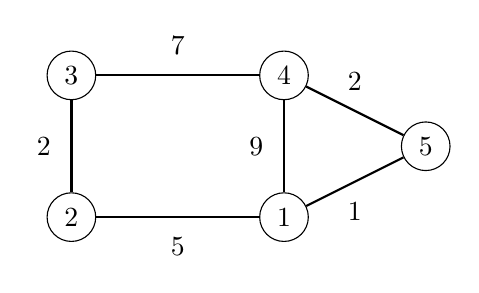
\begin{tikzpicture}[scale=0.9]
\node[draw, circle] (1) at (1,3) {$3$};
\node[draw, circle] (2) at (4,3) {$4$};
\node[draw, circle] (3) at (1,1) {$2$};
\node[draw, circle] (4) at (4,1) {$1$};
\node[draw, circle] (5) at (6,2) {$5$};

\path[draw,thick,-] (1) -- node[font=\small,label=above:7] {} (2);
\path[draw,thick,-] (1) -- node[font=\small,label=left:2] {} (3);
\path[draw,thick,-] (3) -- node[font=\small,label=below:5] {} (4);
\path[draw,thick,-] (2) -- node[font=\small,label=left:9] {} (4);
\path[draw,thick,-] (2) -- node[font=\small,label=above:2] {} (5);
\path[draw,thick,-] (4) -- node[font=\small,label=below:1] {} (5);
\end{tikzpicture}
\end{center}

Na početku je udaljenost od svakog čvora do njega samog $0$,
a udaljenost između čvorova $a$ i $b$ jednaka je $x$
ako postoji brid između čvorova $a$ i $b$ težine $x$.
Sve su ostale udaljenosti beskonačne.

U ovom grafu početni niz izgleda ovako:
\begin{center}
\begin{tabular}{r|rrrrr}
 & 1 & 2 & 3 & 4 & 5 \\
\hline
1 & 0 & 5 & $\infty$ & 9 & 1 \\
2 & 5 & 0 & 2 & $\infty$ & $\infty$ \\
3 & $\infty$ & 2 & 0 & 7 & $\infty$ \\
4 & 9 & $\infty$ & 7 & 0 & 2 \\
5 & 1 & $\infty$ & $\infty$ & 2 & 0 \\
\end{tabular}
\end{center}
\vspace{10pt}
Algoritam se sastoji od uzastopnih prolaza.
U svakom prolazu algoritam odabire novi čvor
koji od tada može služiti kao međučvor na putovima,
a udaljenosti se smanjuju pomoću tog čvora.

U prvom je prolazu čvor 1 novi međučvor.
Postoji novi put između čvorova 2 i 4
duljine 14, jer ih čvor 1 povezuje.
Postoji i novi put
između čvorova 2 i 5 duljine 6.

\begin{center}
\begin{tabular}{r|rrrrr}
 & 1 & 2 & 3 & 4 & 5 \\
\hline
1 & 0 & 5 & $\infty$ & 9 & 1 \\
2 & 5 & 0 & 2 & \textbf{14} & \textbf{6} \\
3 & $\infty$ & 2 & 0 & 7 & $\infty$ \\
4 & 9 & \textbf{14} & 7 & 0 & 2 \\
5 & 1 & \textbf{6} & $\infty$ & 2 & 0 \\
\end{tabular}
\end{center}
\vspace{10pt}

U drugom je prolazu čvor 2 novi međučvor.
Time nastaju novi putovi između čvorova 1 i 3
te između čvorova 3 i 5:

\begin{center}
\begin{tabular}{r|rrrrr}
 & 1 & 2 & 3 & 4 & 5 \\
\hline
1 & 0 & 5 & \textbf{7} & 9 & 1 \\
2 & 5 & 0 & 2 & 14 & 6 \\
3 & \textbf{7} & 2 & 0 & 7 & \textbf{8} \\
4 & 9 & 14 & 7 & 0 & 2 \\
5 & 1 & 6 & \textbf{8} & 2 & 0 \\
\end{tabular}
\end{center}
\vspace{10pt}

U trećem je prolazu čvor 3 novi međučvor.
Postoji novi put između čvorova 2 i 4:

\begin{center}
\begin{tabular}{r|rrrrr}
 & 1 & 2 & 3 & 4 & 5 \\
\hline
1 & 0 & 5 & 7 & 9 & 1 \\
2 & 5 & 0 & 2 & \textbf{9} & 6 \\
3 & 7 & 2 & 0 & 7 & 8 \\
4 & 9 & \textbf{9} & 7 & 0 & 2 \\
5 & 1 & 6 & 8 & 2 & 0 \\
\end{tabular}
\end{center}
\vspace{10pt}

Algoritam tako nastavlja
sve dok svi čvorovi ne budu određeni kao međučvorovi.
Nakon što algoritam završi, niz sadrži
najmanje udaljenosti između bilo koja dva čvora:

\begin{center}
\begin{tabular}{r|rrrrr}
 & 1 & 2 & 3 & 4 & 5 \\
\hline
1 & 0 & 5 & 7 & 3 & 1 \\
2 & 5 & 0 & 2 & 8 & 6 \\
3 & 7 & 2 & 0 & 7 & 8 \\
4 & 3 & 8 & 7 & 0 & 2 \\
5 & 1 & 6 & 8 & 2 & 0 \\
\end{tabular}
\end{center}

Na primjer, niz nam govori da je
najkraća udaljenost između čvorova 2 i 4 jednaka 8.
To odgovara sljedećem putu:

\begin{center}
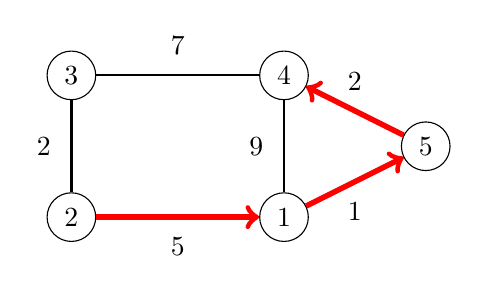
\begin{tikzpicture}[scale=0.9]
\node[draw, circle] (1) at (1,3) {$3$};
\node[draw, circle] (2) at (4,3) {$4$};
\node[draw, circle] (3) at (1,1) {$2$};
\node[draw, circle] (4) at (4,1) {$1$};
\node[draw, circle] (5) at (6,2) {$5$};

\path[draw,thick,-] (1) -- node[font=\small,label=above:7] {} (2);
\path[draw,thick,-] (1) -- node[font=\small,label=left:2] {} (3);
\path[draw,thick,-] (3) -- node[font=\small,label=below:5] {} (4);
\path[draw,thick,-] (2) -- node[font=\small,label=left:9] {} (4);
\path[draw,thick,-] (2) -- node[font=\small,label=above:2] {} (5);
\path[draw,thick,-] (4) -- node[font=\small,label=below:1] {} (5);

\path[draw=red,thick,->,line width=2pt] (3) -- (4);
\path[draw=red,thick,->,line width=2pt] (4) -- (5);
\path[draw=red,thick,->,line width=2pt] (5) -- (2);
\end{tikzpicture}
\end{center}

\subsubsection{Implementacija}

Prednost je
Floyd–Warshallova algoritma to što ga je
jednostavno implementirati.
Sljedeći kod gradi
matricu udaljenosti u kojoj je $\texttt{distance}[a][b]$
najkraća udaljenost između čvorova $a$ i $b$.
Najprije algoritam inicijalizira \texttt{distance}
pomoću matrice susjedstva \texttt{adj} grafa:

\begin{lstlisting}
for (int i = 1; i <= n; i++) {
    for (int j = 1; j <= n; j++) {
        if (i == j) distance[i][j] = 0;
        else if (adj[i][j]) distance[i][j] = adj[i][j];
        else distance[i][j] = INF;
    }
}
\end{lstlisting}
Nakon toga najkraće udaljenosti možemo pronaći ovako:
\begin{lstlisting}
for (int k = 1; k <= n; k++) {
    for (int i = 1; i <= n; i++) {
        for (int j = 1; j <= n; j++) {
            distance[i][j] = min(distance[i][j],
                                   distance[i][k]+distance[k][j]);
        }
    }
}
\end{lstlisting}

Vremenska složenost algoritma je $O(n^3)$,
jer sadrži tri ugniježđene petlje
koje prolaze kroz čvorove grafa.

Budući da je implementacija Floyd–Warshallova
algoritma jednostavna, algoritam može biti
dobar izbor čak i kada je potrebno pronaći samo
jedan najkraći put u grafu.
Međutim, algoritam se može upotrijebiti samo kada je graf
toliko malen da je kubična vremenska složenost dovoljno brza.
